\chapter{Computing Environment Implementation}

\begin{lstlisting}[label=lst:appendix_env_compose, caption=Computing environment docker-compose file]
version: "3.7"
 
networks:
    computing-net:
        name: computing_net
        attachable: true
 
services:
    spark-master:
        image: spark-master:3.0.1-hadoop2.7
        networks:
            - computing-net
        ports:
            - 4040:4040
            - 7077:7077
        volumes:
            - ./conf/spark-master/metrics.properties:/usr/bin/spark/conf/metrics.properties
            - ./conf/spark-master/spark-defaults.conf:/usr/bin/spark/conf/spark-defaults.conf
 
    prometheus:
        image: prom/prometheus
        networks:
            - computing-net
        volumes:
            - ./conf/prometheus/prometheus.yml:/etc/prometheus/prometheus.yml
            - ./conf/prometheus/recording_rules.yml:/etc/prometheus/recording_rules.yml
        command:
            - "--config.file=/etc/prometheus/prometheus.yml"
        ports:
            - "9090:9090"
        depends_on:
            - cadvisor
 
    cadvisor:
        image: google/cadvisor
        networks:
            - computing-net
        ports:
            - "8080:8080"
        volumes:
            - "/:/rootfs:ro"
            - "/var/run:/var/run:ro"
            - "/sys:/sys:ro"
            - "/var/lib/docker/:/var/lib/docker:ro"
            - "/dev/disk/:/dev/disk:ro"
        command:
            - "--docker_only=true"
            - "--logtostderr=true"
        depends_on:
            - spark-master
            - spark-worker
 
    auto-scaler:
        image: auto-scaler:latest
        networks:
            - computing-net
        volumes:
            - "/var/run/docker.sock:/var/run/docker.sock:ro"
            - ./conf/auto-scaler/config.yml:/etc/autoscaler/config.yml
        command:
            - '--config=/etc/autoscaler/config.yml'
        depends_on:
            - prometheus
\end{lstlisting}

\chapter{Apache Spark Cluster Implementation}

% Base image dockerfile
\begin{lstlisting}[label=lst:appendix_spark_base_dockerfile, caption=Apache Spark base image Dockerfile]
FROM nvidia/cuda:11.0-devel-ubuntu16.04
 
LABEL maintainer="marcel.pascal.stolin@ipa.fraunhofer.de"
 
ARG SPARK_VERSION
ARG HADOOP_VERSION
 
# Install all important packages
RUN apt-get update -qy && \
    apt-get install -y openjdk-8-jre-headless procps python3 python3-pip curl
 
# Install Apache Spark
RUN mkdir /usr/bin/spark/ && \
    curl https://ftp-stud.hs-esslingen.de/pub/Mirrors/ftp.apache.org/dist/spark/spark-${SPARK_VERSION}/spark-${SPARK_VERSION}-bin-hadoop${HADOOP_VERSION}.tgz -o spark.tgz && \
    tar -xf spark.tgz && \
    mv spark-${SPARK_VERSION}-bin-hadoop${HADOOP_VERSION}/* /usr/bin/spark/ && \
    rm -rf spark.tgz && \
    rm -rf spark-${SPARK_VERSION}-bin-hadoop${HADOOP_VERSION}/
 
# Add GPU discovery script
RUN mkdir /opt/sparkRapidsPlugin/
COPY getGpusResources.sh /opt/sparkRapidsPlugin/getGpusResources.sh
ENV SPARK_RAPIDS_DIR=/opt/sparkRapidsPlugin
 
# Install cuDF and RAPIDS
RUN curl -o ${SPARK_RAPIDS_DIR}/cudf-0.15-cuda11.jar https://repo1.maven.org/maven2/ai/rapids/cudf/0.15/cudf-0.15-cuda11.jar
RUN curl -o ${SPARK_RAPIDS_DIR}/rapids-4-spark_2.12-0.2.0.jar https://repo1.maven.org/maven2/com/nvidia/rapids-4-spark_2.12/0.2.0/rapids-4-spark_2.12-0.2.0.jar
ENV SPARK_CUDF_JAR=${SPARK_RAPIDS_DIR}/cudf-0.15-cuda11.jar
ENV SPARK_RAPIDS_PLUGIN_JAR=${SPARK_RAPIDS_DIR}/rapids-4-spark_2.12-0.2.0.jar
 
# Set all environment variables
ENV JAVA_HOME=/usr/lib/jvm/java-8-openjdk-amd64
ENV SPARK_HOME /usr/bin/spark
ENV SPARK_NO_DAEMONIZE true
ENV PYSPARK_DRIVER_PYTHON python3
ENV PYSPARK_PYTHON python3
ENV PATH /usr/bin/spark/bin:/usr/bin/spark/sbin:$PATH
 
WORKDIR ${SPARK_HOME}
\end{lstlisting}


% Master image dockerfile
\begin{lstlisting}[label=lst:appendix_spark_master_dockerfile, caption=Apache Spark master image Dockerfile]
ARG SPARK_VERSION
ARG HADOOP_VERSION
 
FROM spark-base:$SPARK_VERSION-hadoop$HADOOP_VERSION
 
LABEL maintainer="marcel.pascal.stolin@ipa.fraunhofer.de"
 
# Set ports
ENV SPARK_MASTER_PORT 7077
ENV SPARK_MASTER_WEBUI_PORT 4040
 
EXPOSE 4040 7077
 
# Start master-node in standalone mode
ENTRYPOINT [ "sbin/start-master.sh" ]
\end{lstlisting}


% Worker image Dockerfile
\begin{lstlisting}[label=lst:appendix_spark_worker_dockerfile, caption=Apache Spark worker image Dockerfile]
ARG SPARK_VERSION
ARG HADOOP_VERSION
 
FROM spark-base:$SPARK_VERSION-hadoop$HADOOP_VERSION
 
LABEL maintainer="marcel.pascal.stolin@ipa.fraunhofer.de"
 
# Add spark-env
COPY spark-env.sh ${SPARK_HOME}/conf/spark-env.sh
 
# Set port
ENV SPARK_WORKER_WEBUI_PORT 4041
 
EXPOSE 4041
 
# Start worker-node
ENTRYPOINT ./sbin/start-slave.sh ${SPARK_MASTER_URI}
\end{lstlisting}


% GPU discovery script
\begin{lstlisting}[label=lst:appendix_spark_gpu-discovery, caption=GPU discovery script - Source: \url{https://github.com/apache/spark/blob/v3.0.1/examples/src/main/scripts/getGpusResources.sh} (Accessed: 2021-01-03), language=bash]
#!/usr/bin/env bash

#
# Licensed to the Apache Software Foundation (ASF) under one or more
# contributor license agreements.  See the NOTICE file distributed with
# this work for additional information regarding copyright ownership.
# The ASF licenses this file to You under the Apache License, Version 2.0
# (the "License"); you may not use this file except in compliance with
# the License.  You may obtain a copy of the License at
#
#    http://www.apache.org/licenses/LICENSE-2.0
#
# Unless required by applicable law or agreed to in writing, software
# distributed under the License is distributed on an "AS IS" BASIS,
# WITHOUT WARRANTIES OR CONDITIONS OF ANY KIND, either express or implied.
# See the License for the specific language governing permissions and
# limitations under the License.
#

# This script is a basic example script to get resource information about NVIDIA GPUs.
# It assumes the drivers are properly installed and the nvidia-smi command is available.
# It is not guaranteed to work on all setups so please test and customize as needed
# for your environment. It can be passed into SPARK via the config
# spark.{driver/executor}.resource.gpu.discoveryScript to allow the driver or executor to discover
# the GPUs it was allocated. It assumes you are running within an isolated container where the
# GPUs are allocated exclusively to that driver or executor.
# It outputs a JSON formatted string that is expected by the
# spark.{driver/executor}.resource.gpu.discoveryScript config.
#
# Example output: {"name": "gpu", "addresses":["0","1","2","3","4","5","6","7"]}

ADDRS=`nvidia-smi --query-gpu=index --format=csv,noheader | sed -e ':a' -e 'N' -e'$!ba' -e 's/\n/","/g'`
echo {\"name\": \"gpu\", \"addresses\":[\"$ADDRS\"]}
\end{lstlisting}

% Custom submit script
\begin{lstlisting}[label=lst:appendix_spark-submit_script, caption=Custom submit script, language=sh]
#!/bin/bash
 
DRIVER_MEMORY=${DRIVER_MEMORY-4g}
EXECUTOR_MEMORY=${EXECUTOR_MEMORY-8g}
 
if [ "$CPU_ONLY" == "true" ]
    then
    echo "Submit Spark app with CPU only"
 
    $SPARK_HOME/bin/spark-submit \
        --master $SPARK_MASTER_URI \
        --driver-memory $DRIVER_MEMORY \
        --executor-memory $EXECUTOR_MEMORY \
        --conf spark.driver.extraClassPath=${SPARK_CUDF_JAR}:${JAR_RAPIDS}:${LIBS_PATH}/xgboost4j_3.0-1.3.0-0.1.0.jar:${LIBS_PATH}/xgboost4j-spark_3.0-1.3.0-0.1.0.jar \
        --conf spark.executor.extraClassPath=${SPARK_CUDF_JAR}:${JAR_RAPIDS}:${LIBS_PATH}/xgboost4j_3.0-1.3.0-0.1.0.jar:${LIBS_PATH}/xgboost4j-spark_3.0-1.3.0-0.1.0.jar \
        --jars ${SPARK_CUDF_JAR},${LIBS_PATH}/xgboost4j-spark_3.0-1.3.0-0.1.0.jar,${LIBS_PATH}/xgboost4j_3.0-1.3.0-0.1.0.jar,${JAR_RAPIDS} \
        --py-files ${LIBS_PATH}/xgboost4j-spark_3.0-1.3.0-0.1.0.jar,/tank/data/users/chh-ms/spark-xgboost-examples/examples/apps/python/samples.zip \
        $@
else
    echo "Submit Spark app with GPU acceleration"
 
    RAPIDS_GPU_ALLOC_FRACTION=${RAPIDS_GPU_ALLOC_FRACTION-1}
    RAPIDS_INCOMPATIBLE_OPS=${RAPIDS_INCOMPATIBLE_OPS-"false"}
    RAPIDS_DEBUG=${RAPIDS_DEBUG-"NONE"}
    RAPIDS_GPU_POOL=${RAPIDS_GPU_POOL-"ARENA"}
 
    $SPARK_HOME/bin/spark-submit \
        --master $SPARK_MASTER_URI \
        --driver-memory $DRIVER_MEMORY \
        --executor-memory $EXECUTOR_MEMORY \
        --conf spark.plugins=com.nvidia.spark.SQLPlugin \
        --conf spark.rapids.memory.gpu.pool=$RAPIDS_GPU_POOL \
        --conf spark.rapids.memory.gpu.allocFraction=$RAPIDS_GPU_ALLOC_FRACTION \
        --conf spark.rapids.sql.incompatibleOps.enabled=$RAPIDS_INCOMPATIBLE_OPS \
        --conf spark.rapids.memory.gpu.debug=$RAPIDS_DEBUG \
        --conf spark.task.resource.gpu.amount=1 \
        --conf spark.executor.resource.gpu.amount=1 \
        --conf spark.driver.extraClassPath=${SPARK_CUDF_JAR}:${JAR_RAPIDS}:${LIBS_PATH}/xgboost4j_3.0-1.3.0-0.1.0.jar:${LIBS_PATH}/xgboost4j-spark_3.0-1.3.0-0.1.0.jar \
        --conf spark.executor.extraClassPath=${SPARK_CUDF_JAR}:${JAR_RAPIDS}:${LIBS_PATH}/xgboost4j_3.0-1.3.0-0.1.0.jar:${LIBS_PATH}/xgboost4j-spark_3.0-1.3.0-0.1.0.jar \
        --jars ${SPARK_CUDF_JAR},${LIBS_PATH}/xgboost4j-spark_3.0-1.3.0-0.1.0.jar,${LIBS_PATH}/xgboost4j_3.0-1.3.0-0.1.0.jar,${JAR_RAPIDS} \
        --py-files ${LIBS_PATH}/xgboost4j-spark_3.0-1.3.0-0.1.0.jar,/tank/data/users/chh-ms/spark-xgboost-examples/examples/apps/python/samples.zip \
        $@  
fi
\end{lstlisting}


\section{Evaluation Data}

\begin{figure}[h]
\centering
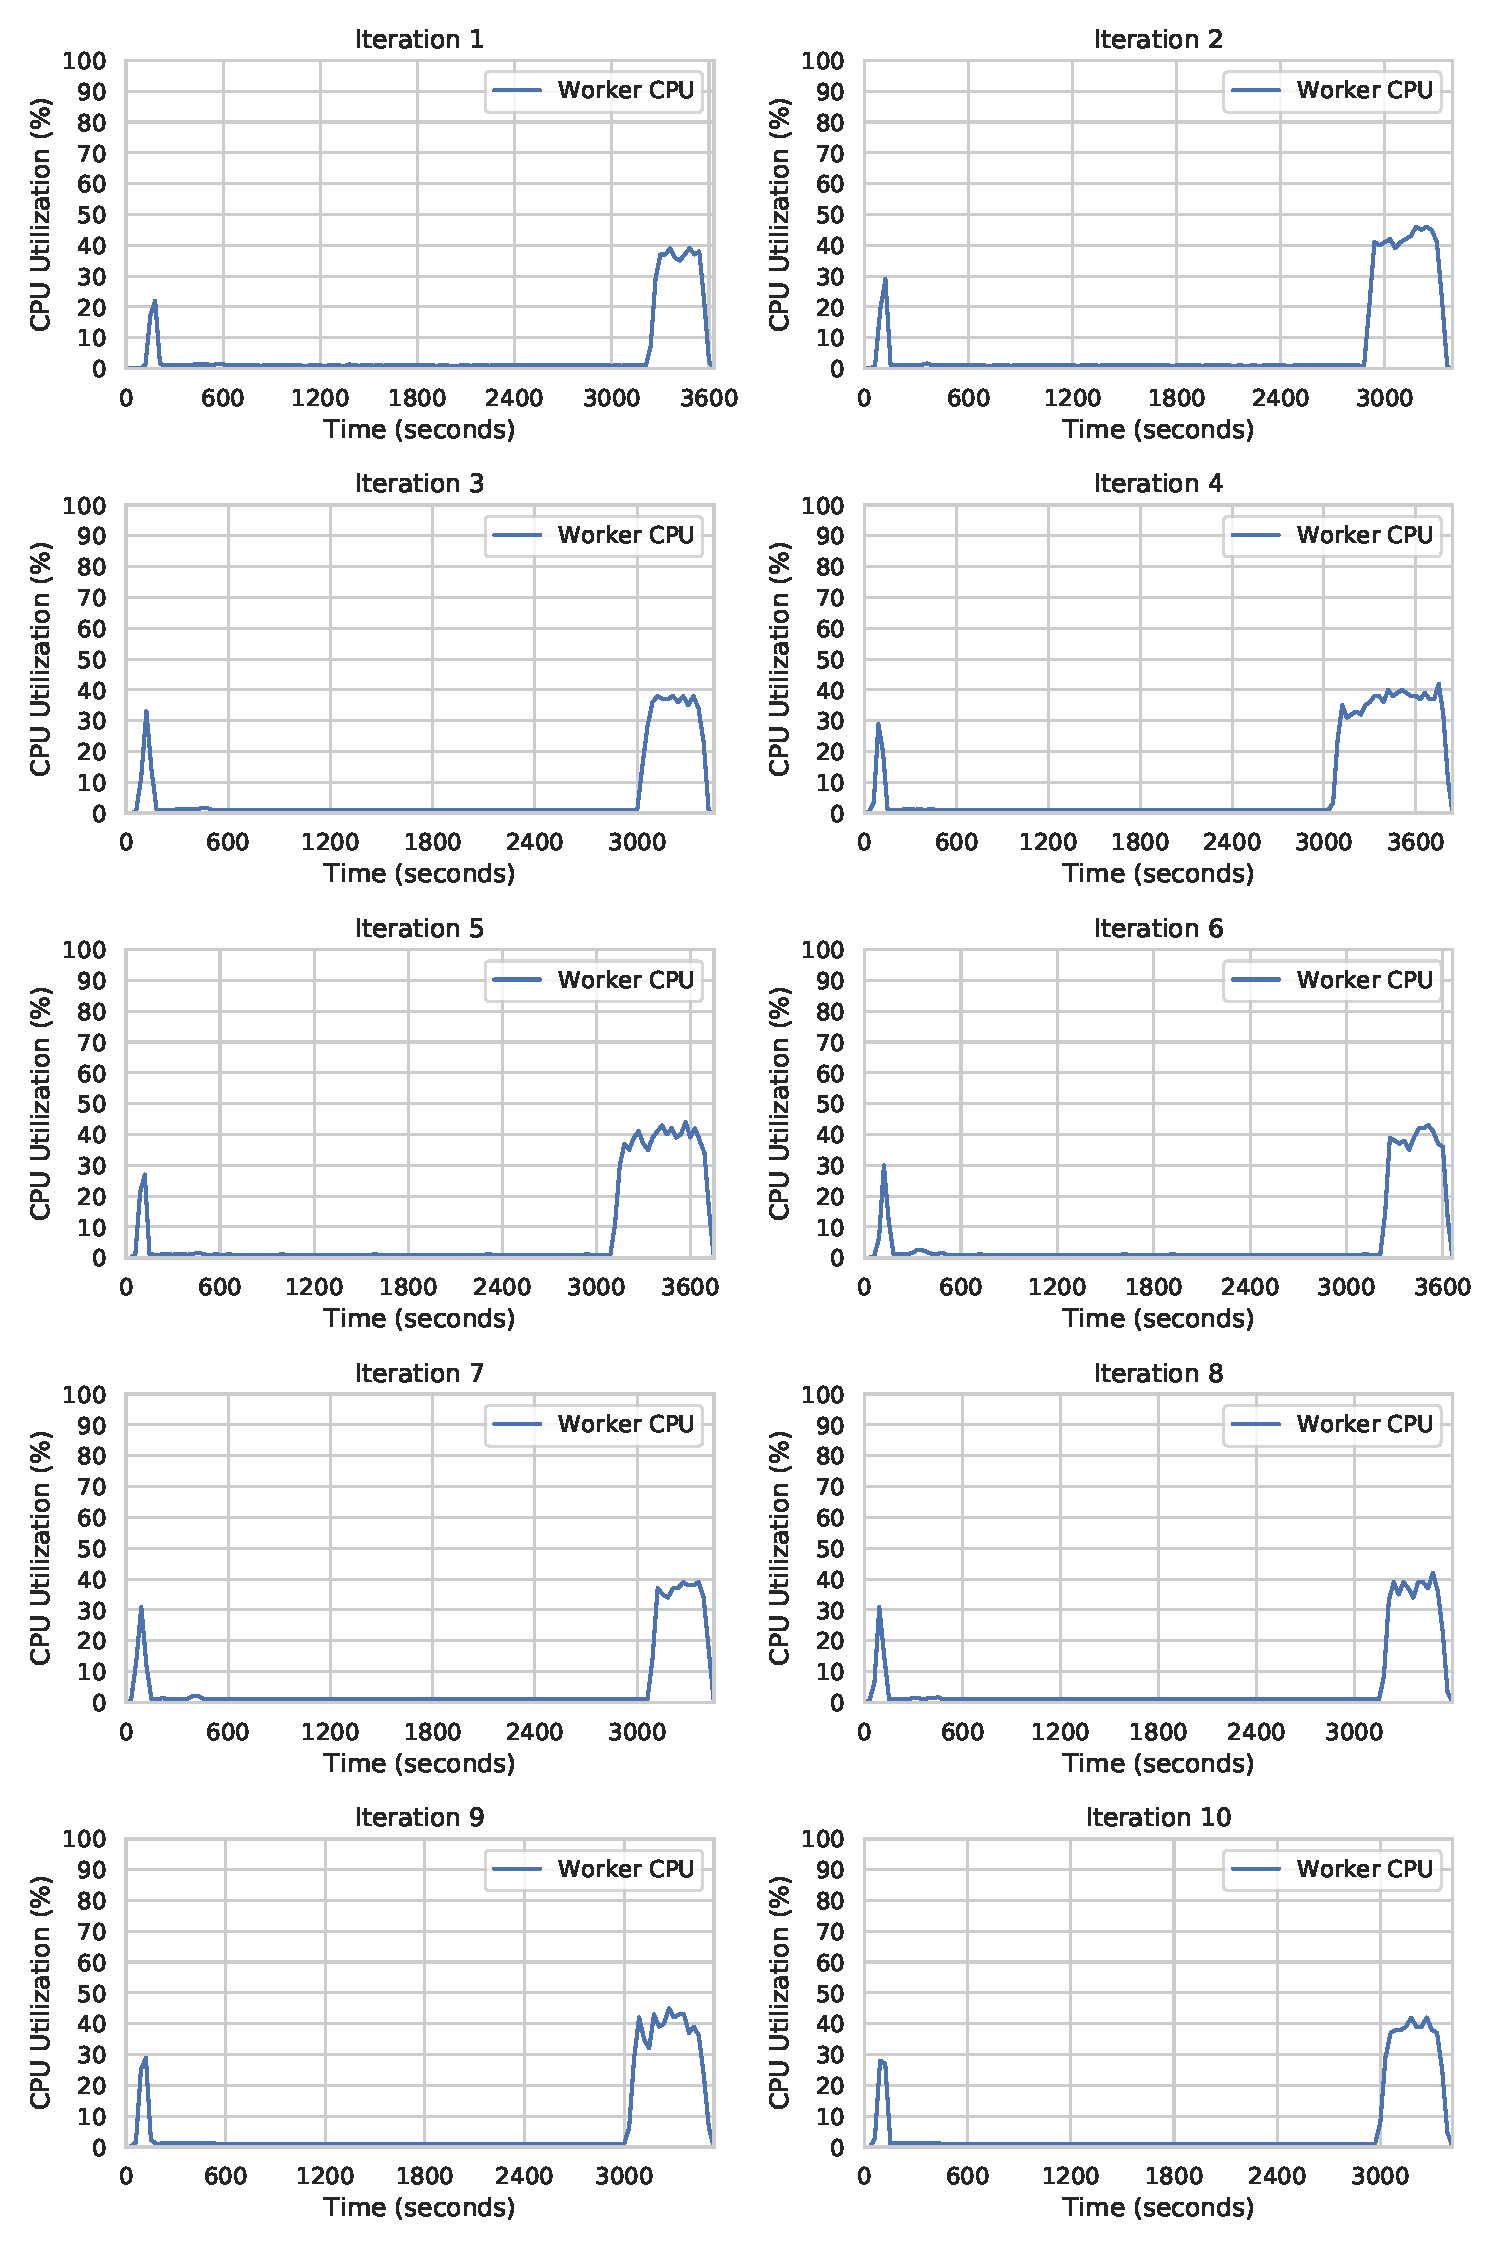
\includegraphics[scale=0.53]{images/07_evaluation/mortgage/mortgage_1_worker_cpu_performance}
\caption{Classification algorithm performance evaluation of the computing environment with 1 Apache Spark worker}
\label{fig:07_mortgage_static-cpu_results}
\end{figure}

\begin{figure}[h]
\centering
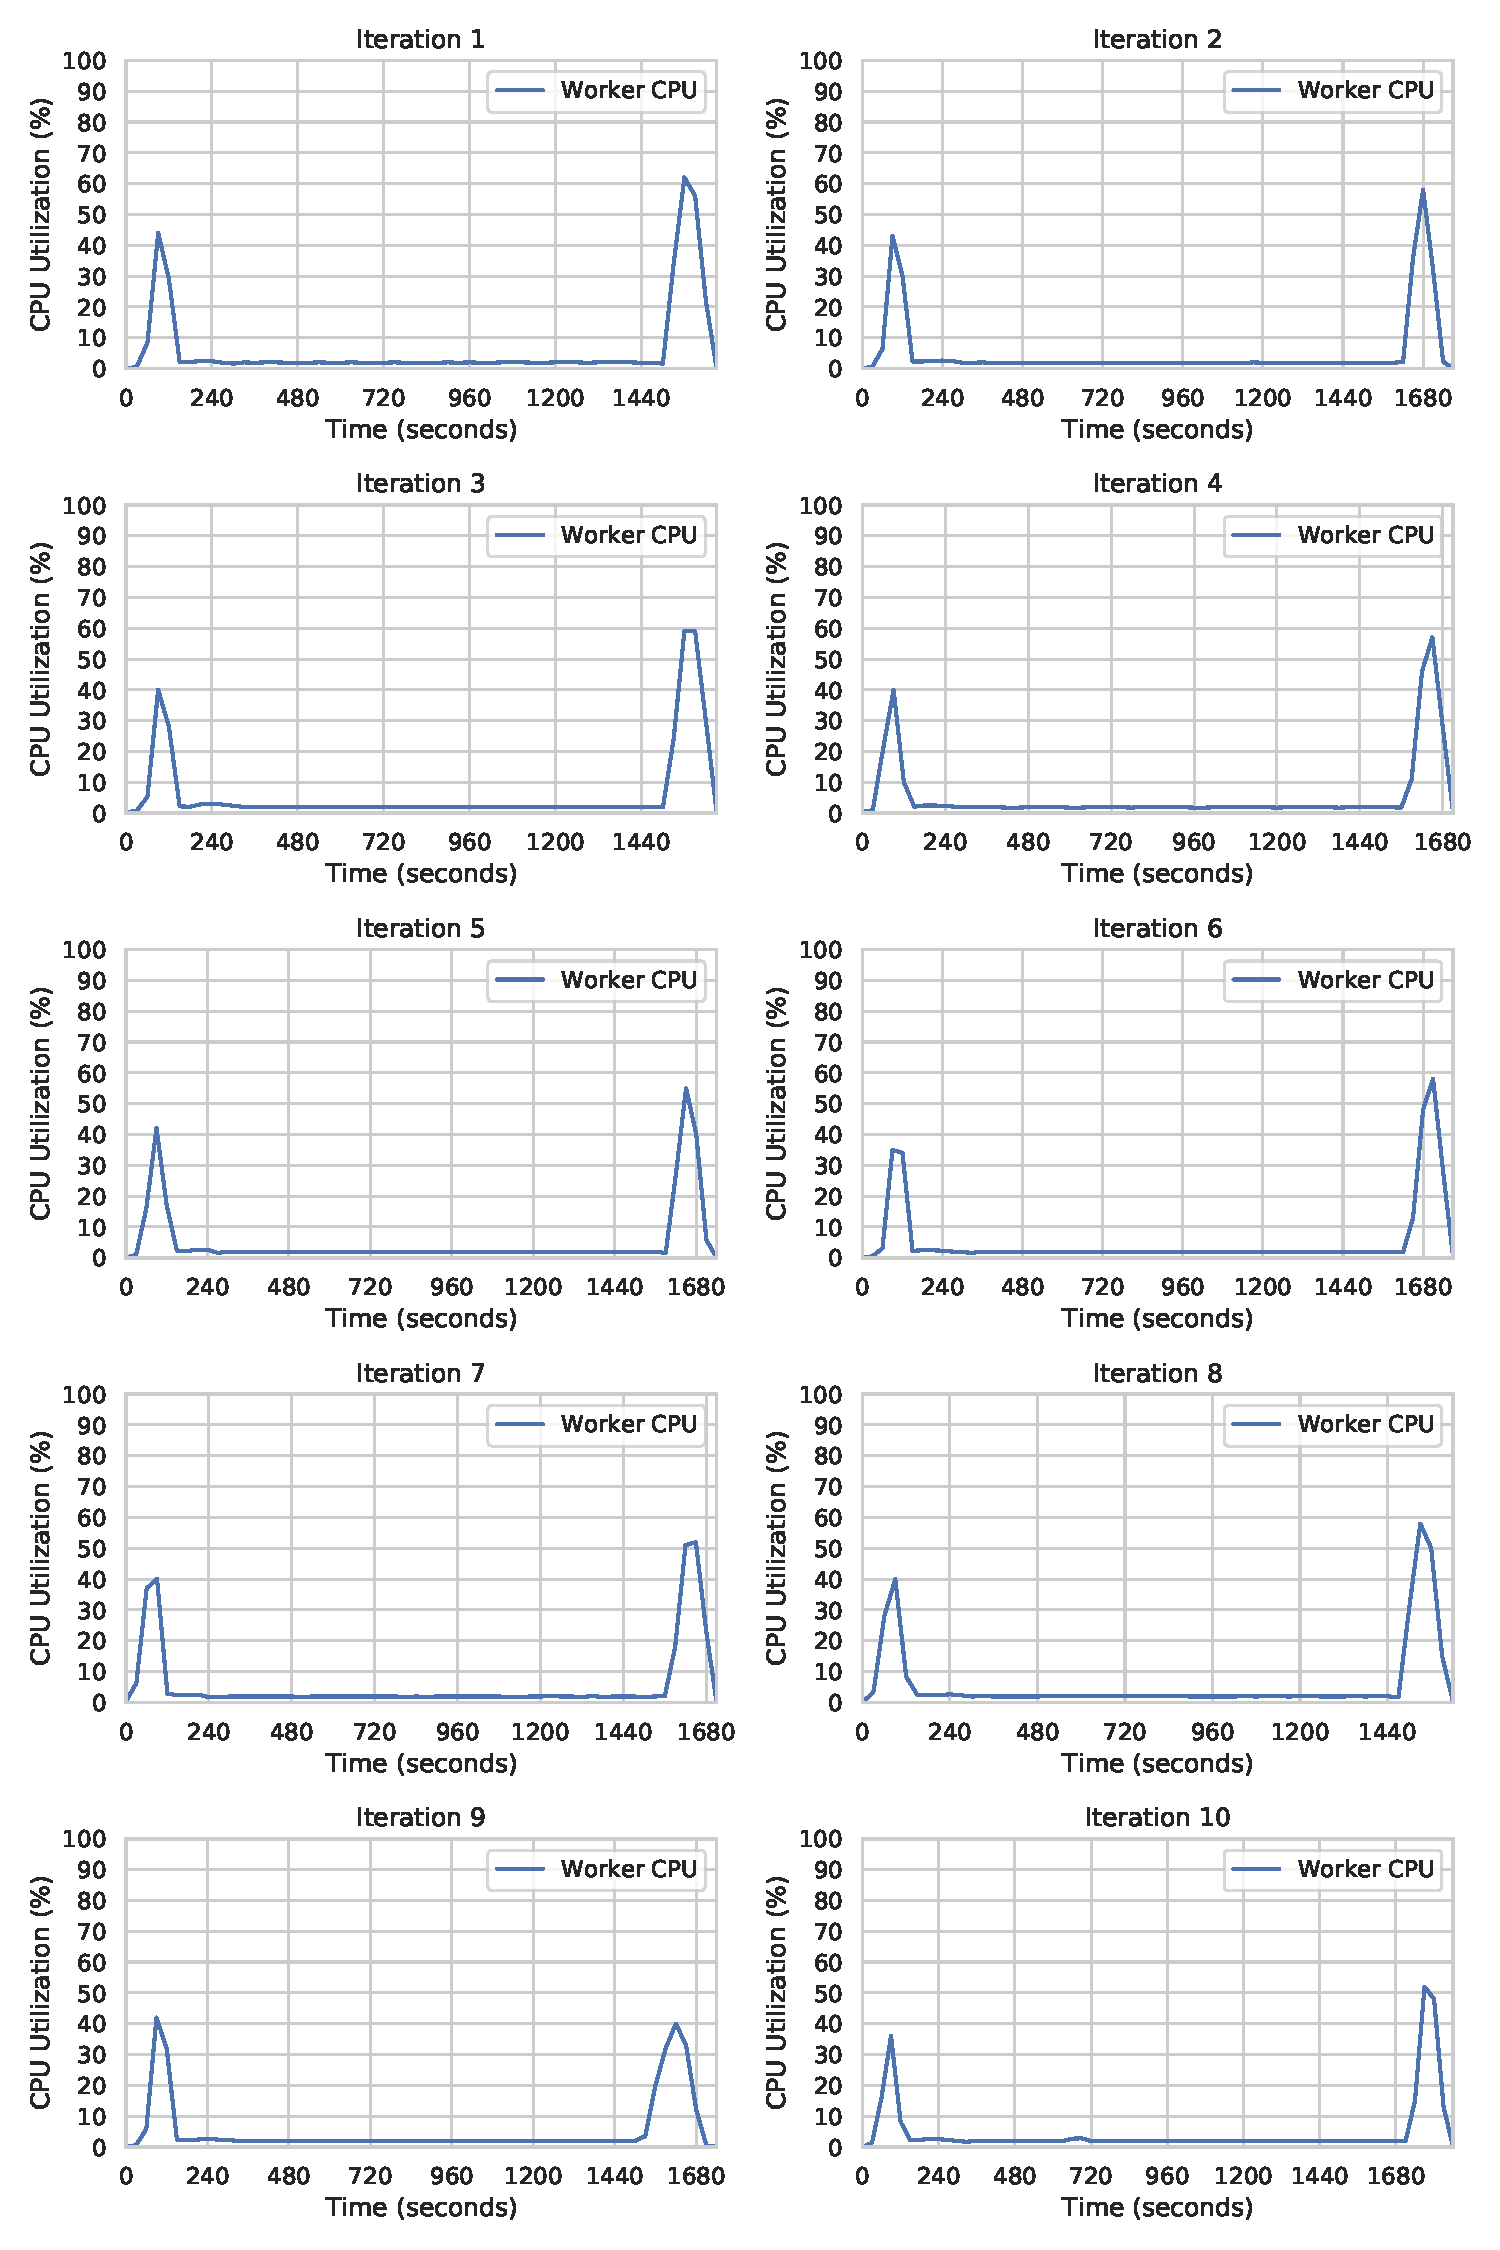
\includegraphics[scale=0.53]{images/07_evaluation/mortgage/mortgage_2_worker_cpu_performance}
\caption{Classification algorithm performance evaluation of the computing environment with 2 Apache Spark worker}
\label{fig:07_mortgage_static-cpu_results}
\end{figure}

\begin{figure}[h]
\centering
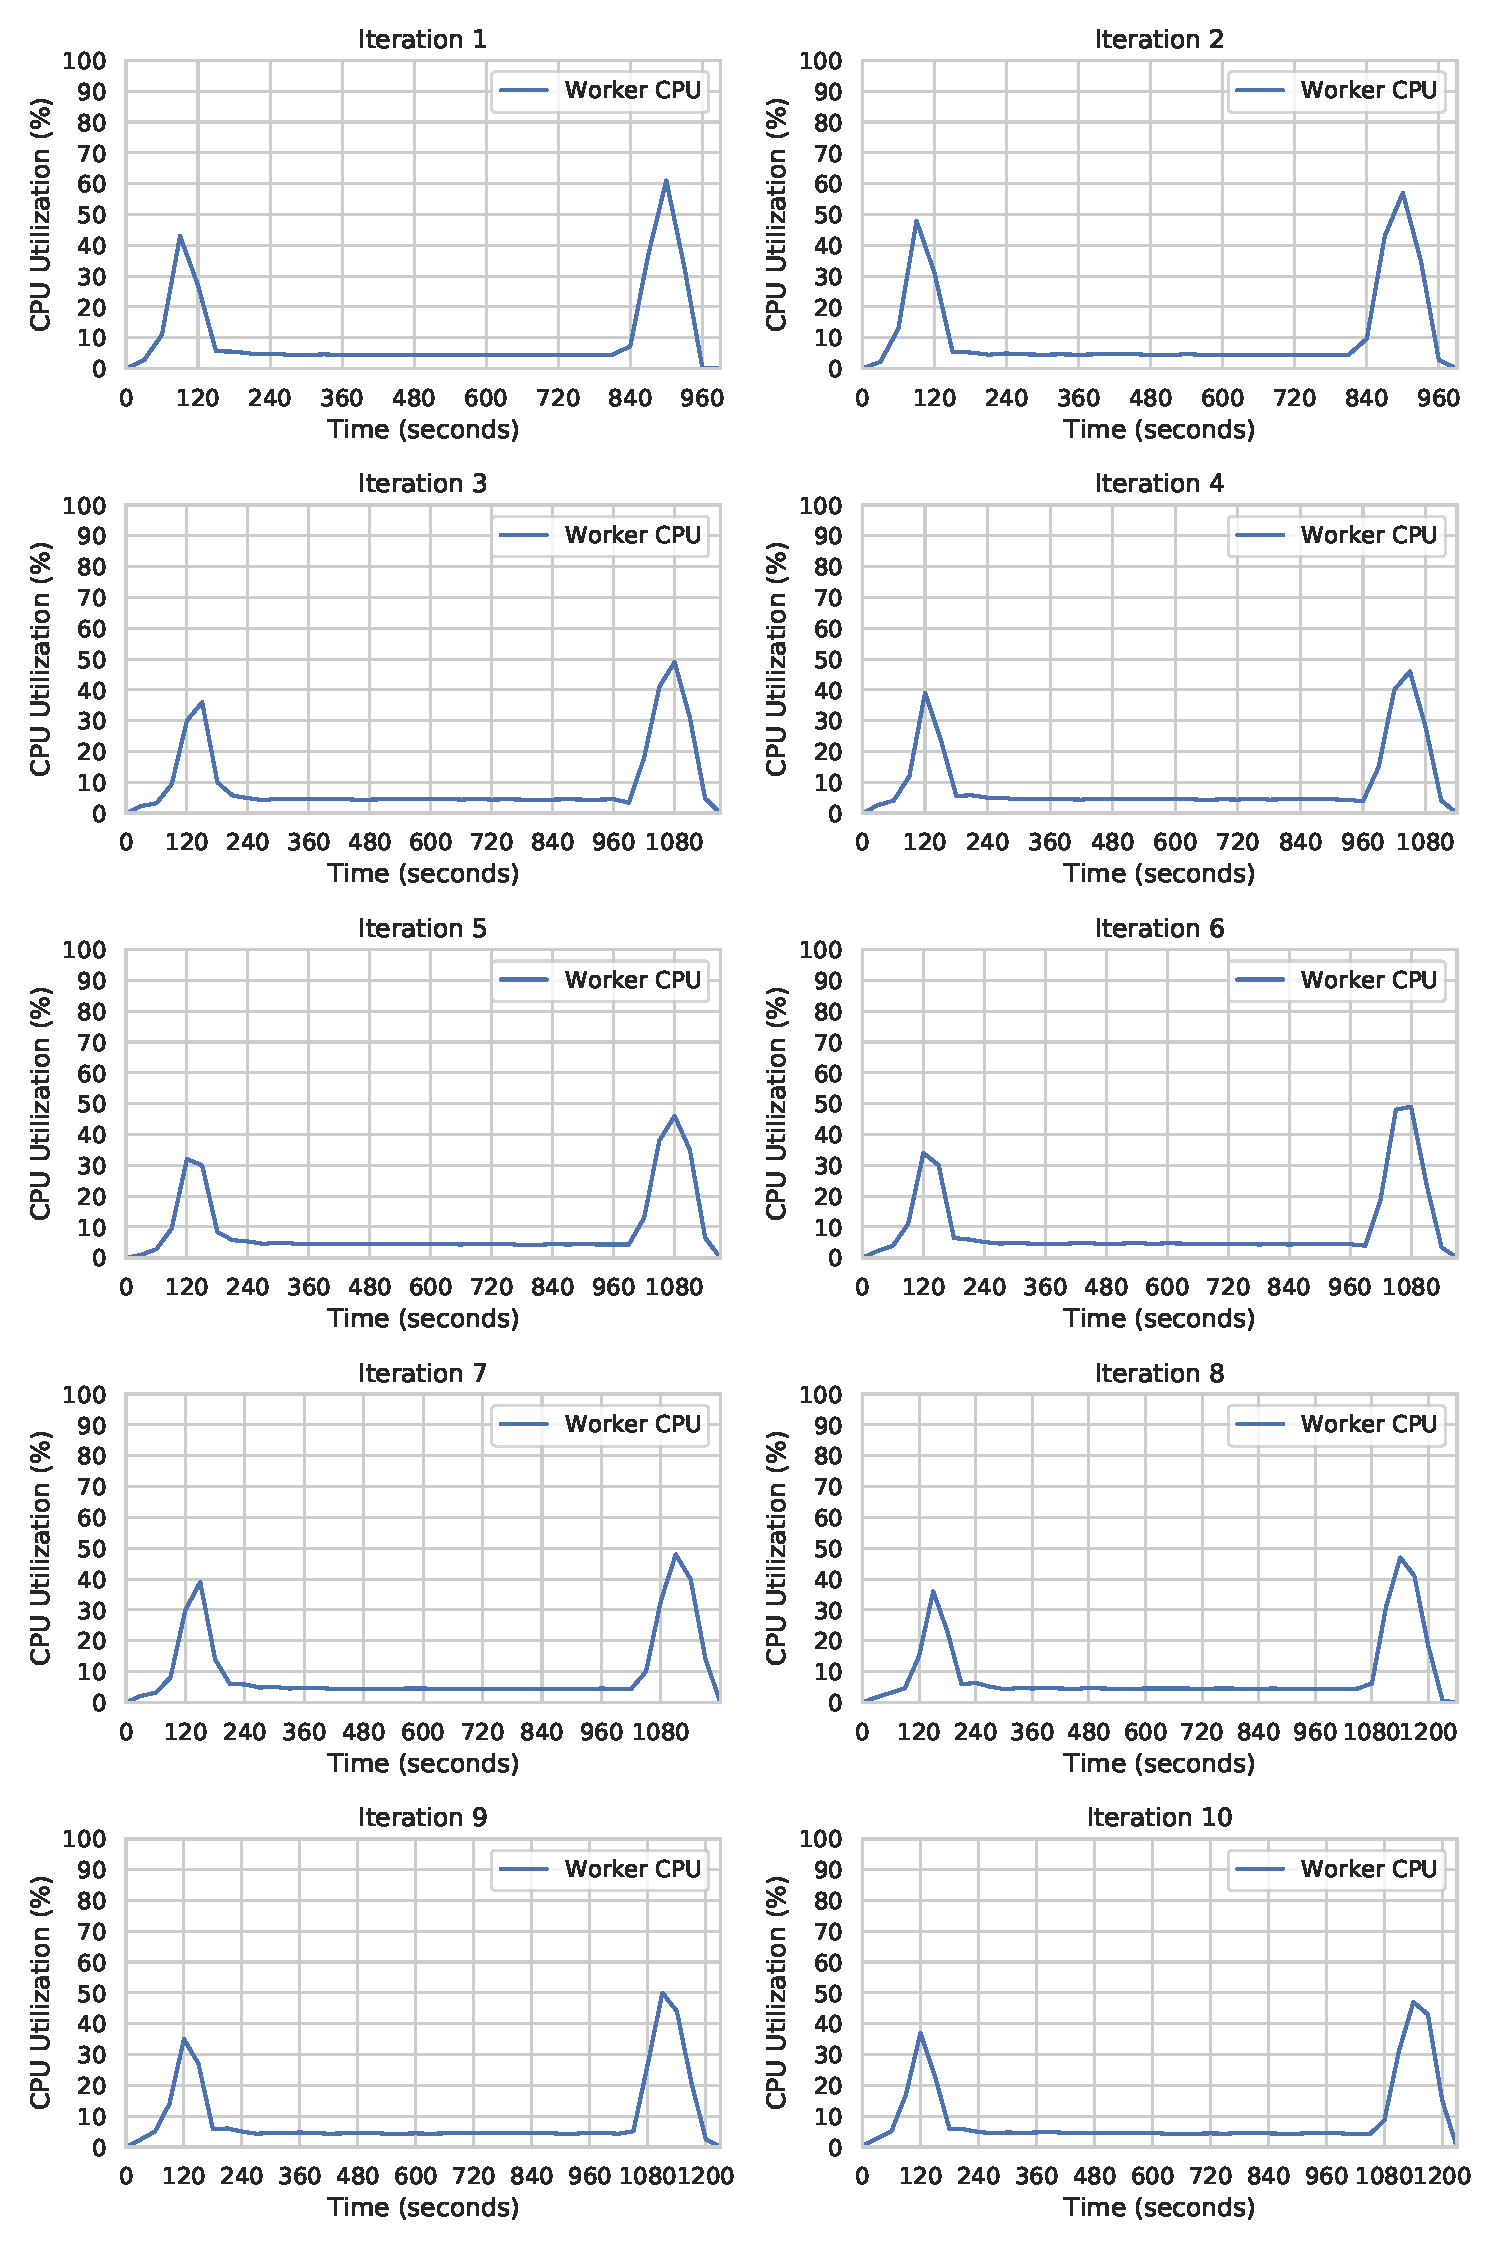
\includegraphics[scale=0.53]{images/07_evaluation/mortgage/mortgage_5_worker_cpu_performance}
\caption{Classification algorithm performance evaluation of the computing environment with 5 Apache Spark worker}
\label{fig:07_mortgage_static-cpu_results}
\end{figure}

\begin{figure}[h]
\centering
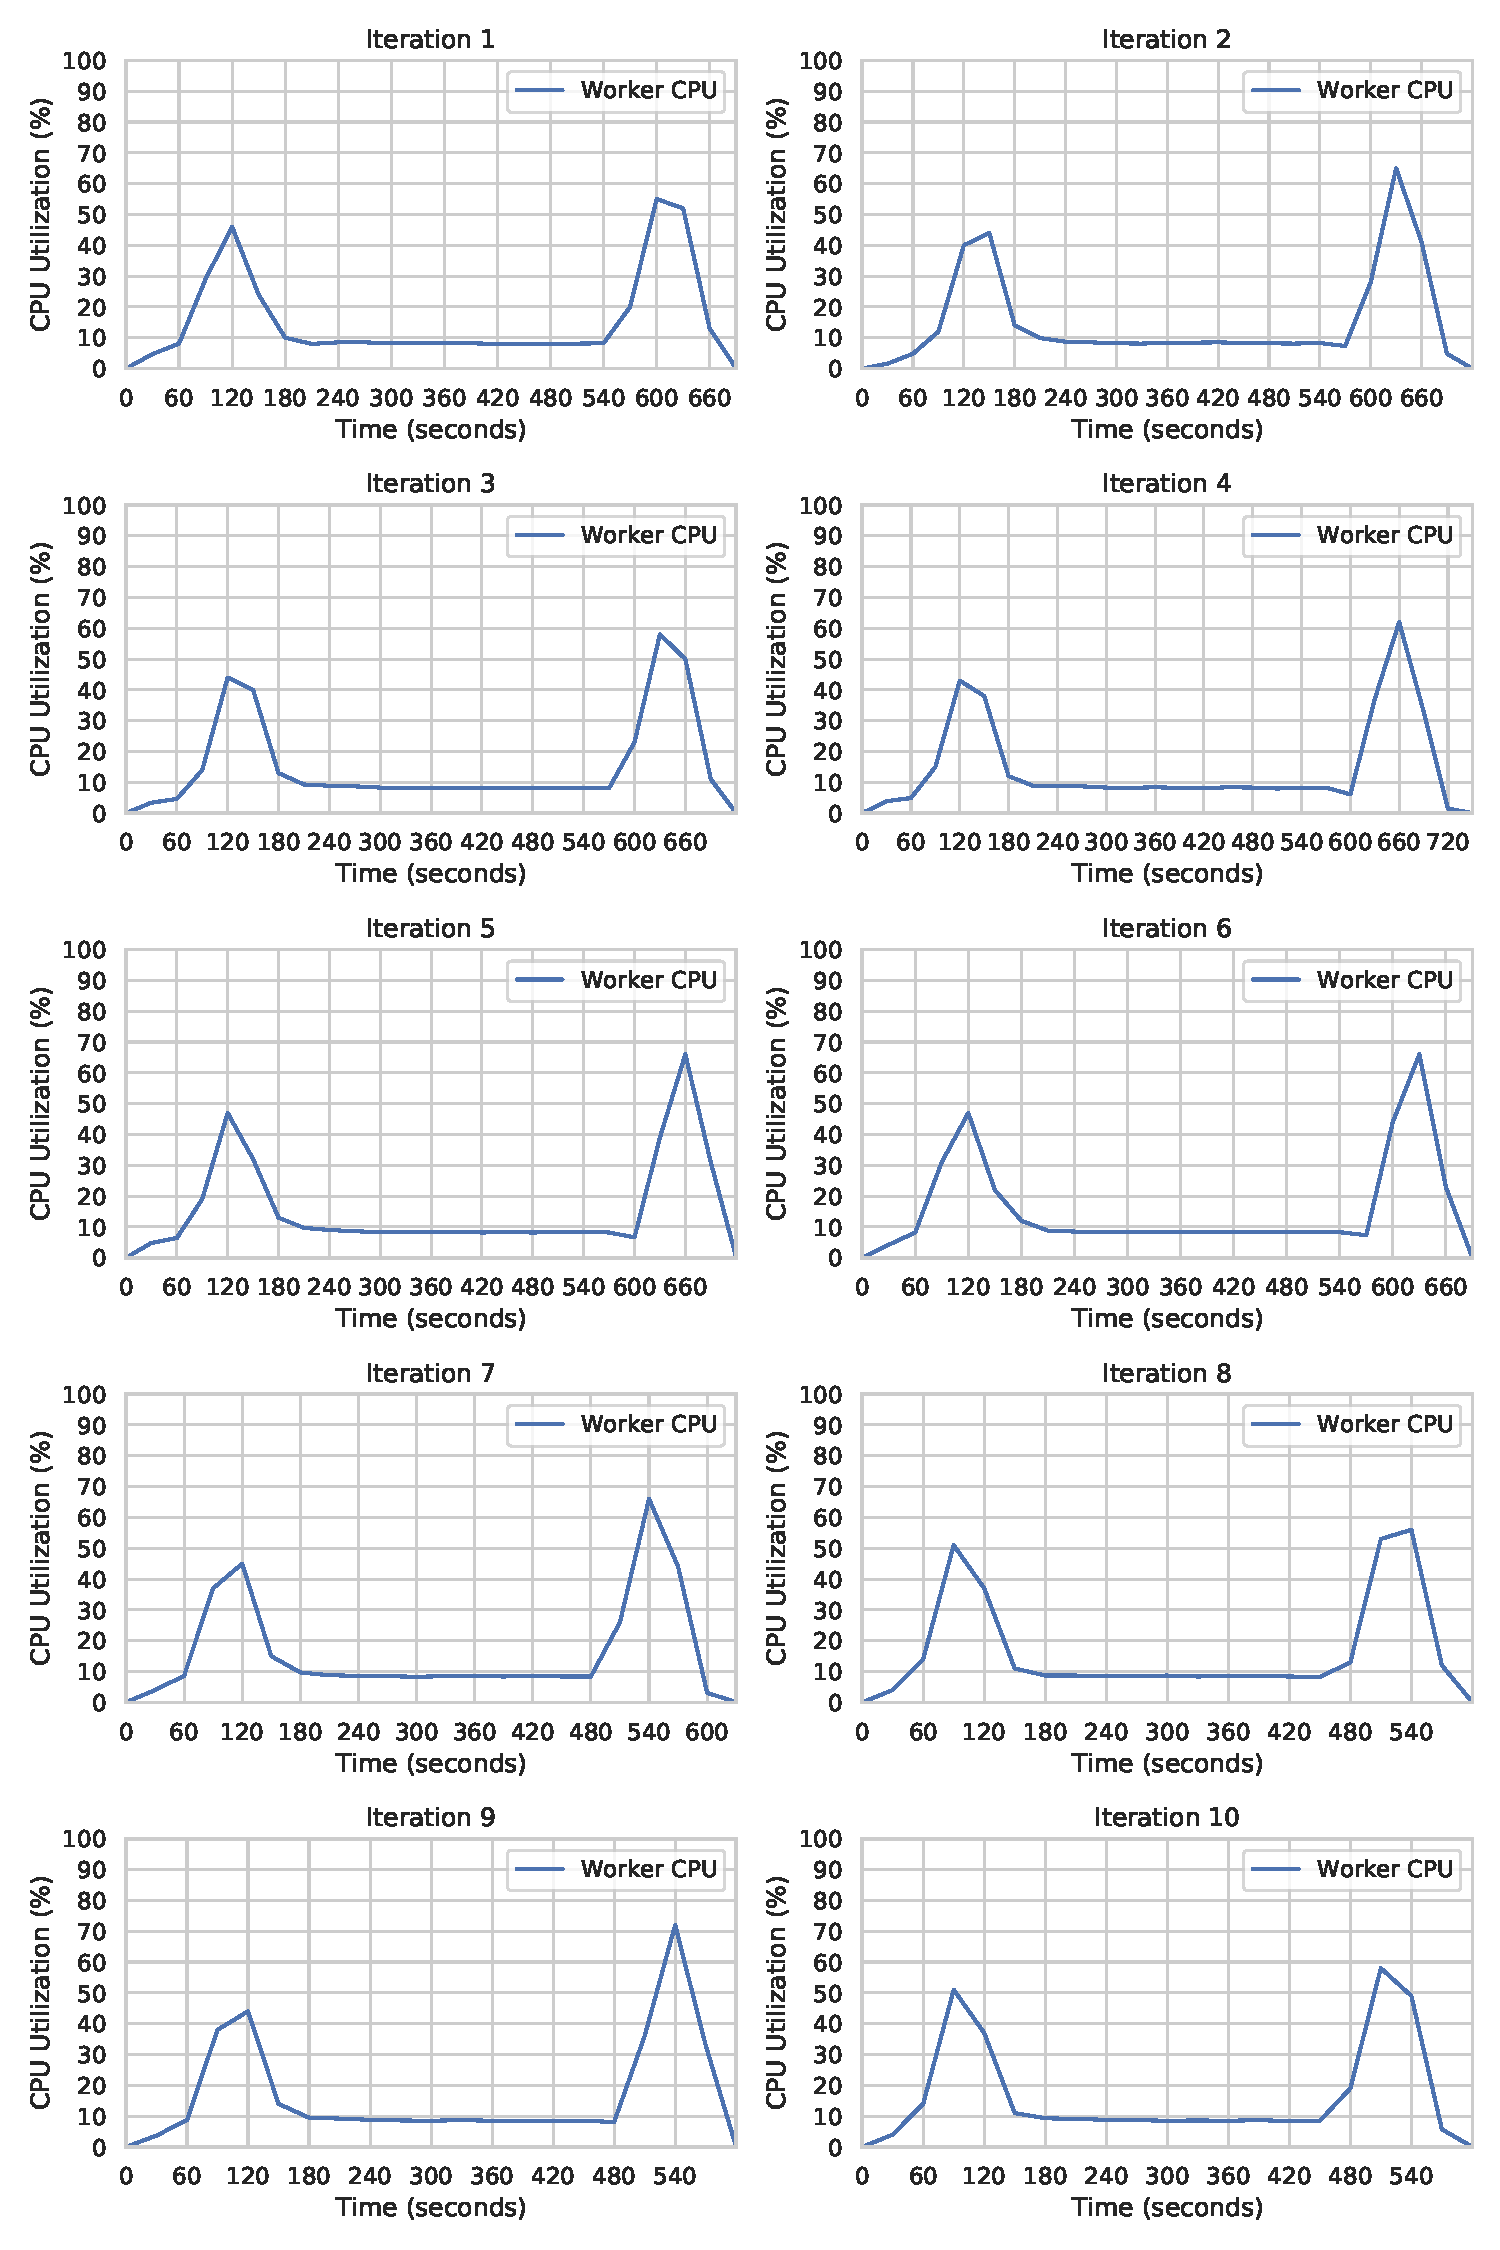
\includegraphics[scale=0.53]{images/07_evaluation/mortgage/mortgage_10_worker_cpu_performance}
\caption{Classification algorithm performance evaluation of the computing environment with 10 Apache Spark worker}
\label{fig:07_mortgage_static-cpu_results}
\end{figure}

\begin{figure}[h]
\centering
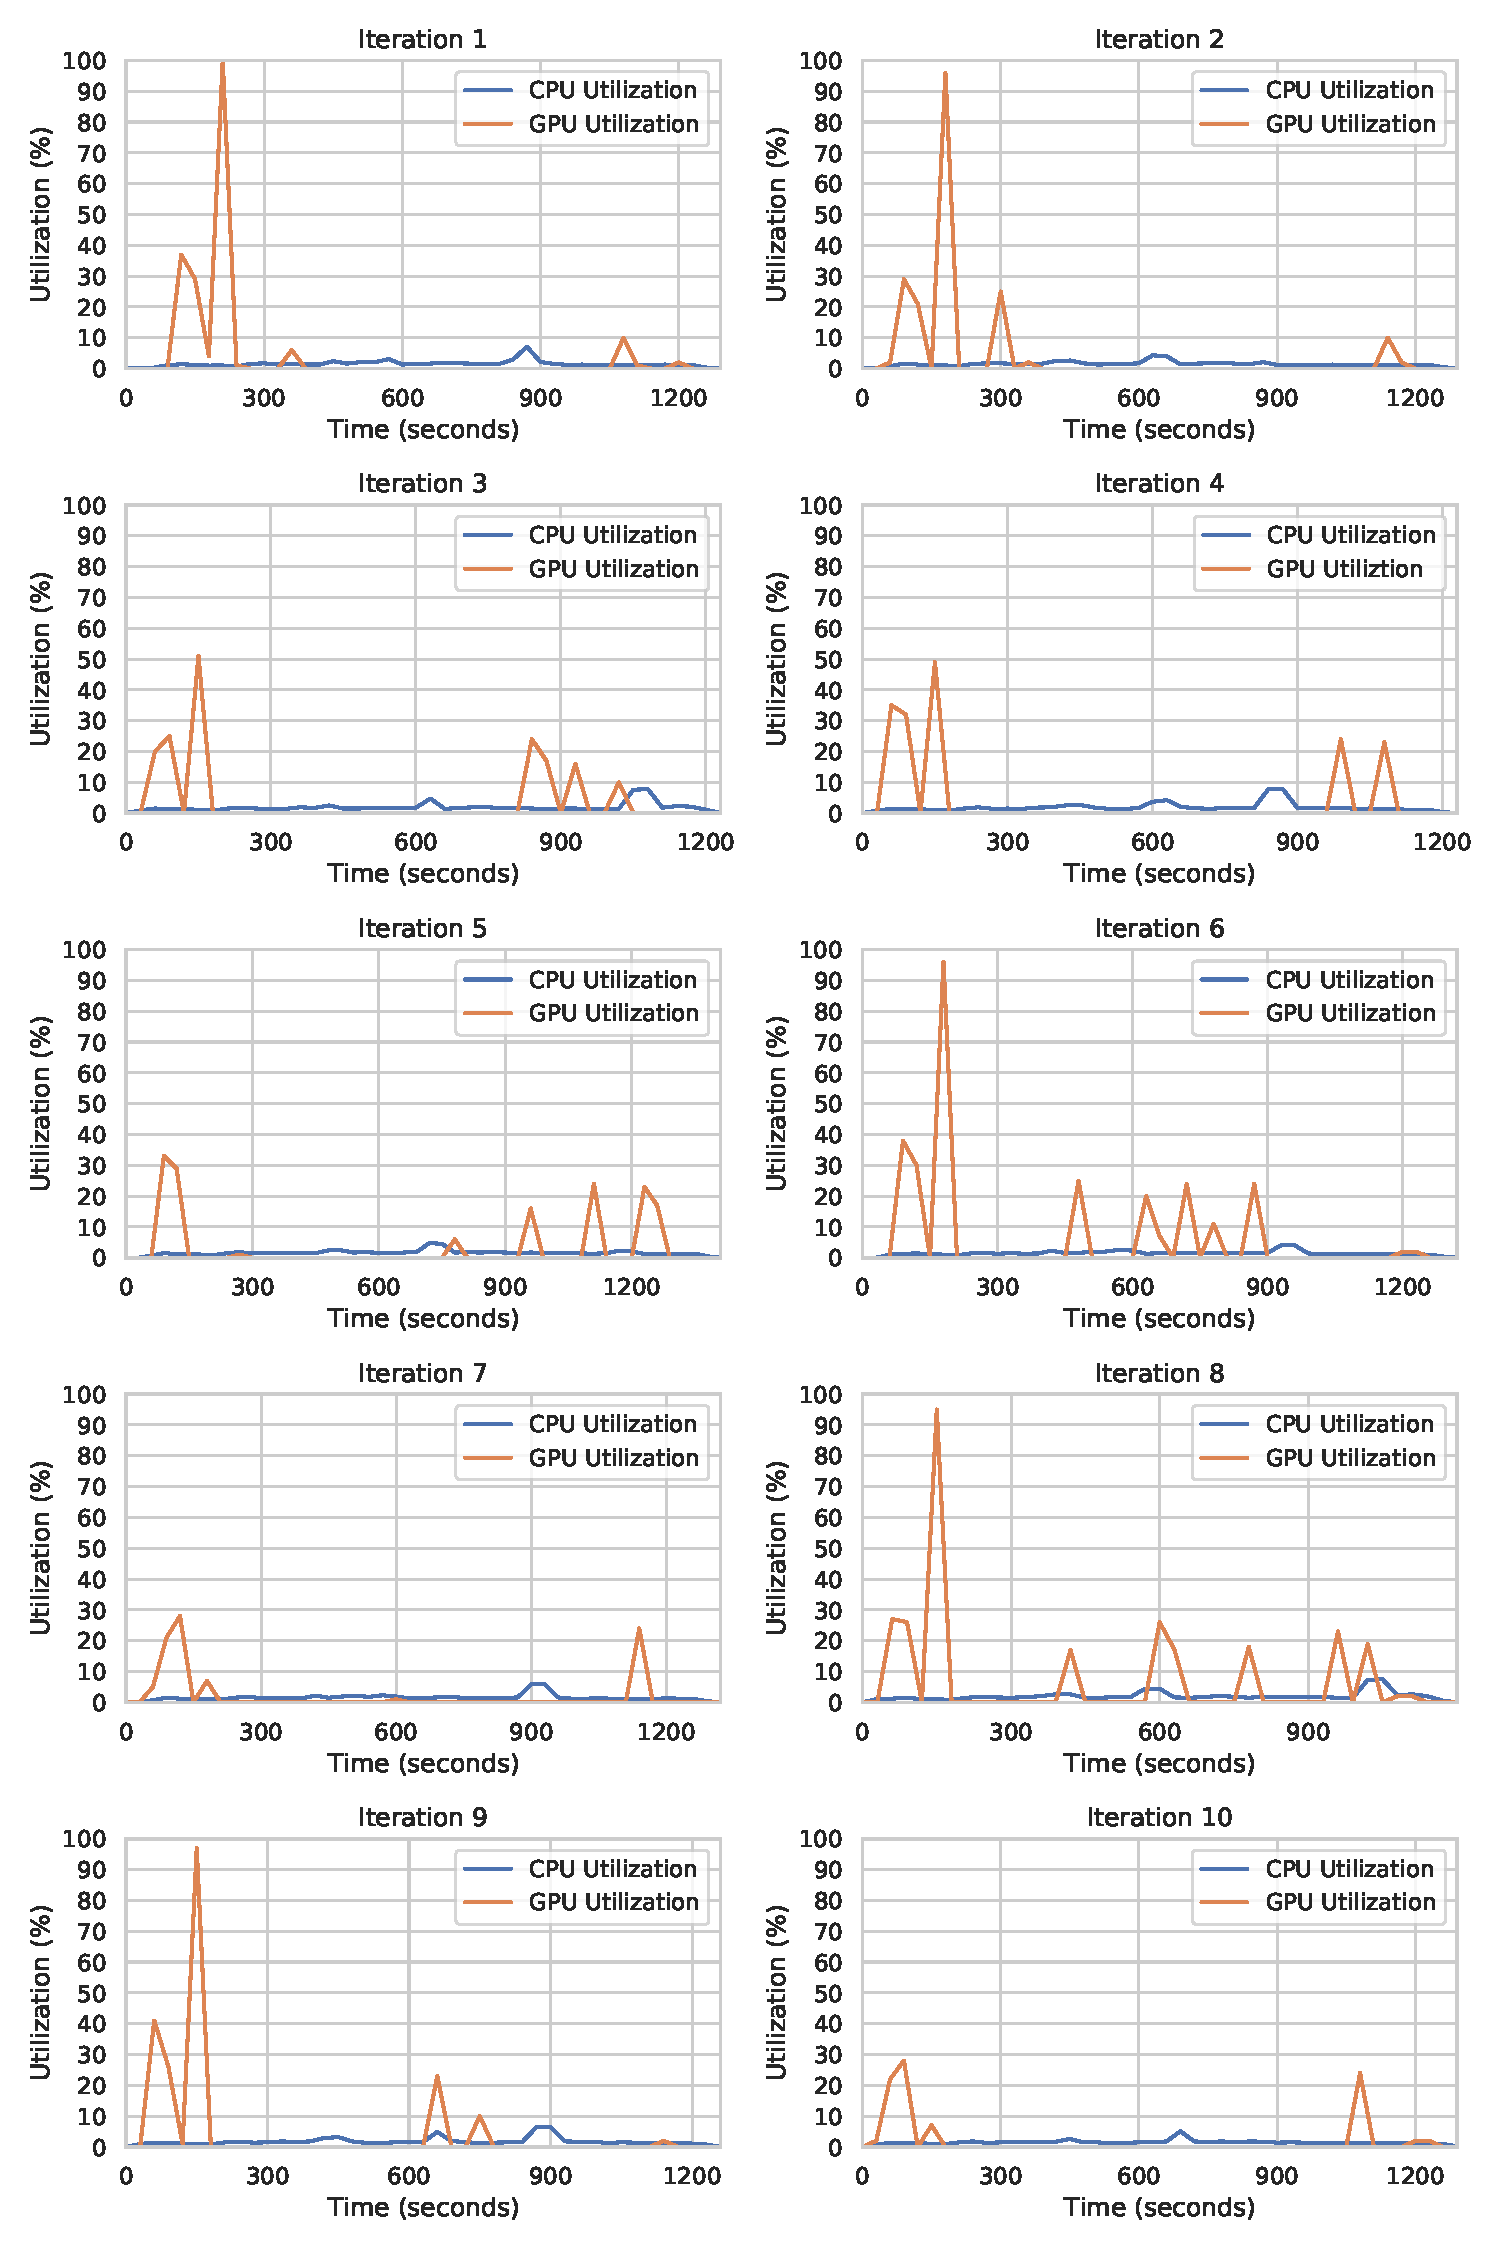
\includegraphics[scale=0.53]{images/07_evaluation/mortgage/mortgage_gpu1_performance}
\caption{Classification algorithm performance evaluation of the computing environment with 1 Apache Spark worker and GPU acceleration enabled}
\label{fig:07_mortgage_static-cpu_results}
\end{figure}

\begin{figure}[h]
\centering
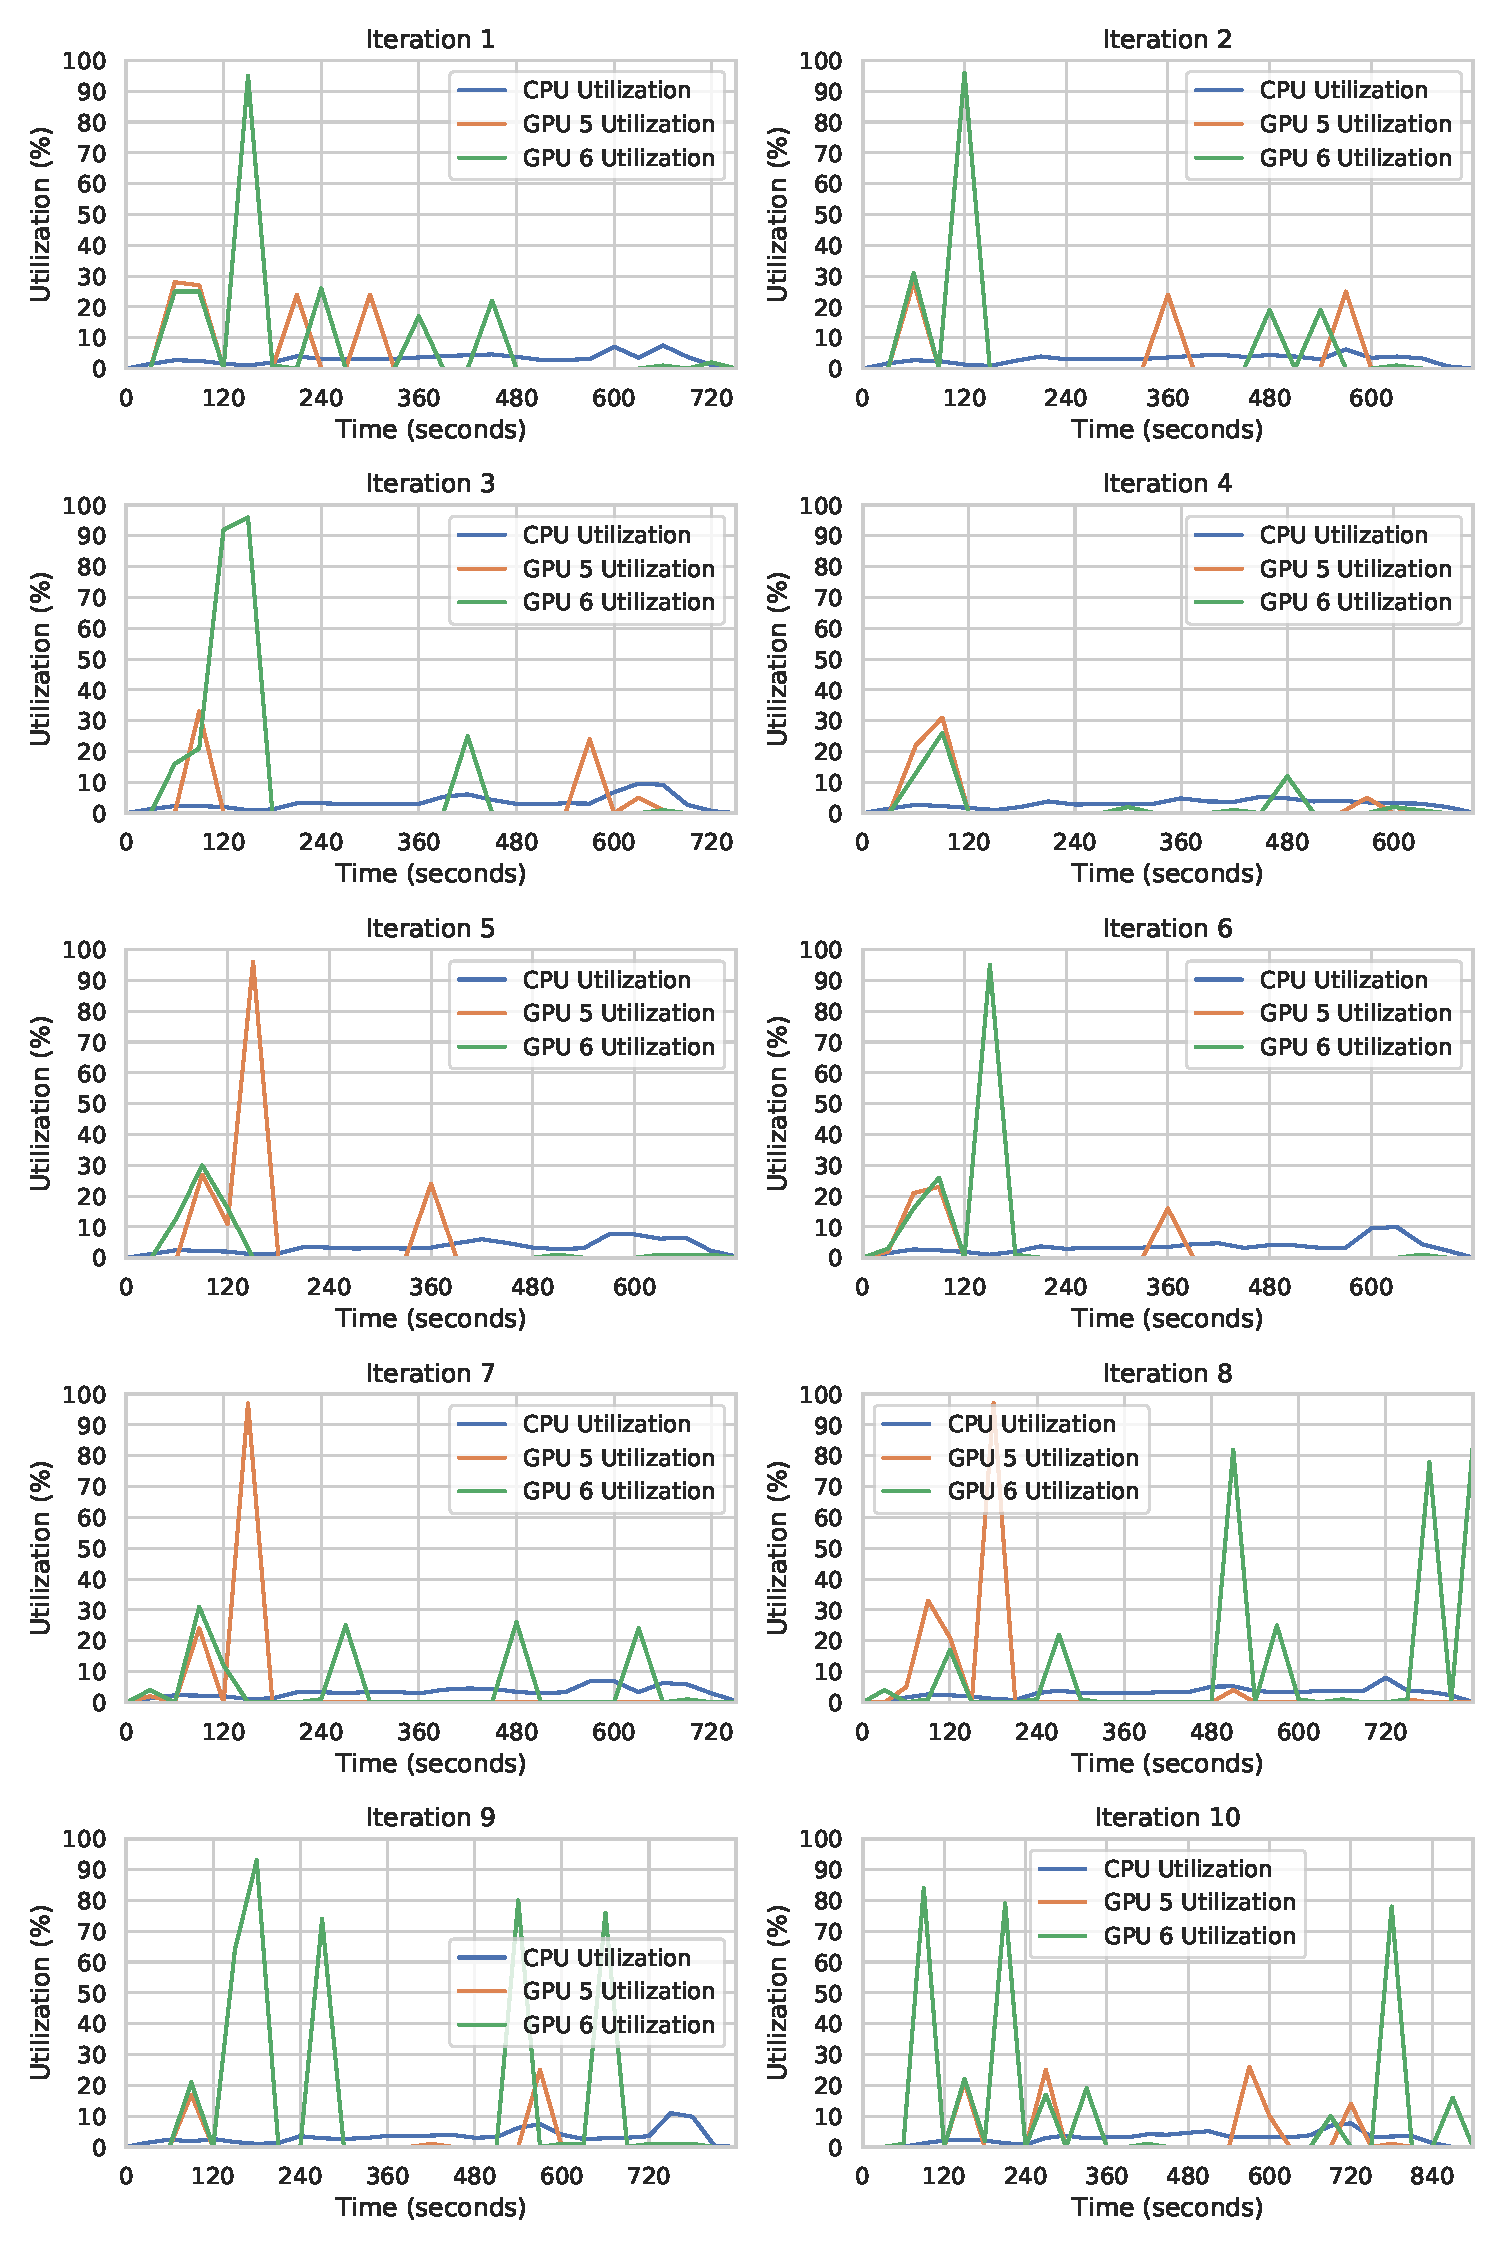
\includegraphics[scale=0.53]{images/07_evaluation/mortgage/mortgage_gpu2_performance}
\caption{Classification algorithm performance evaluation of the computing environment with 2 Apache Spark worker and GPU acceleration enabled}
\label{fig:07_mortgage_static-cpu_results}
\end{figure}

\begin{figure}[h]
\centering
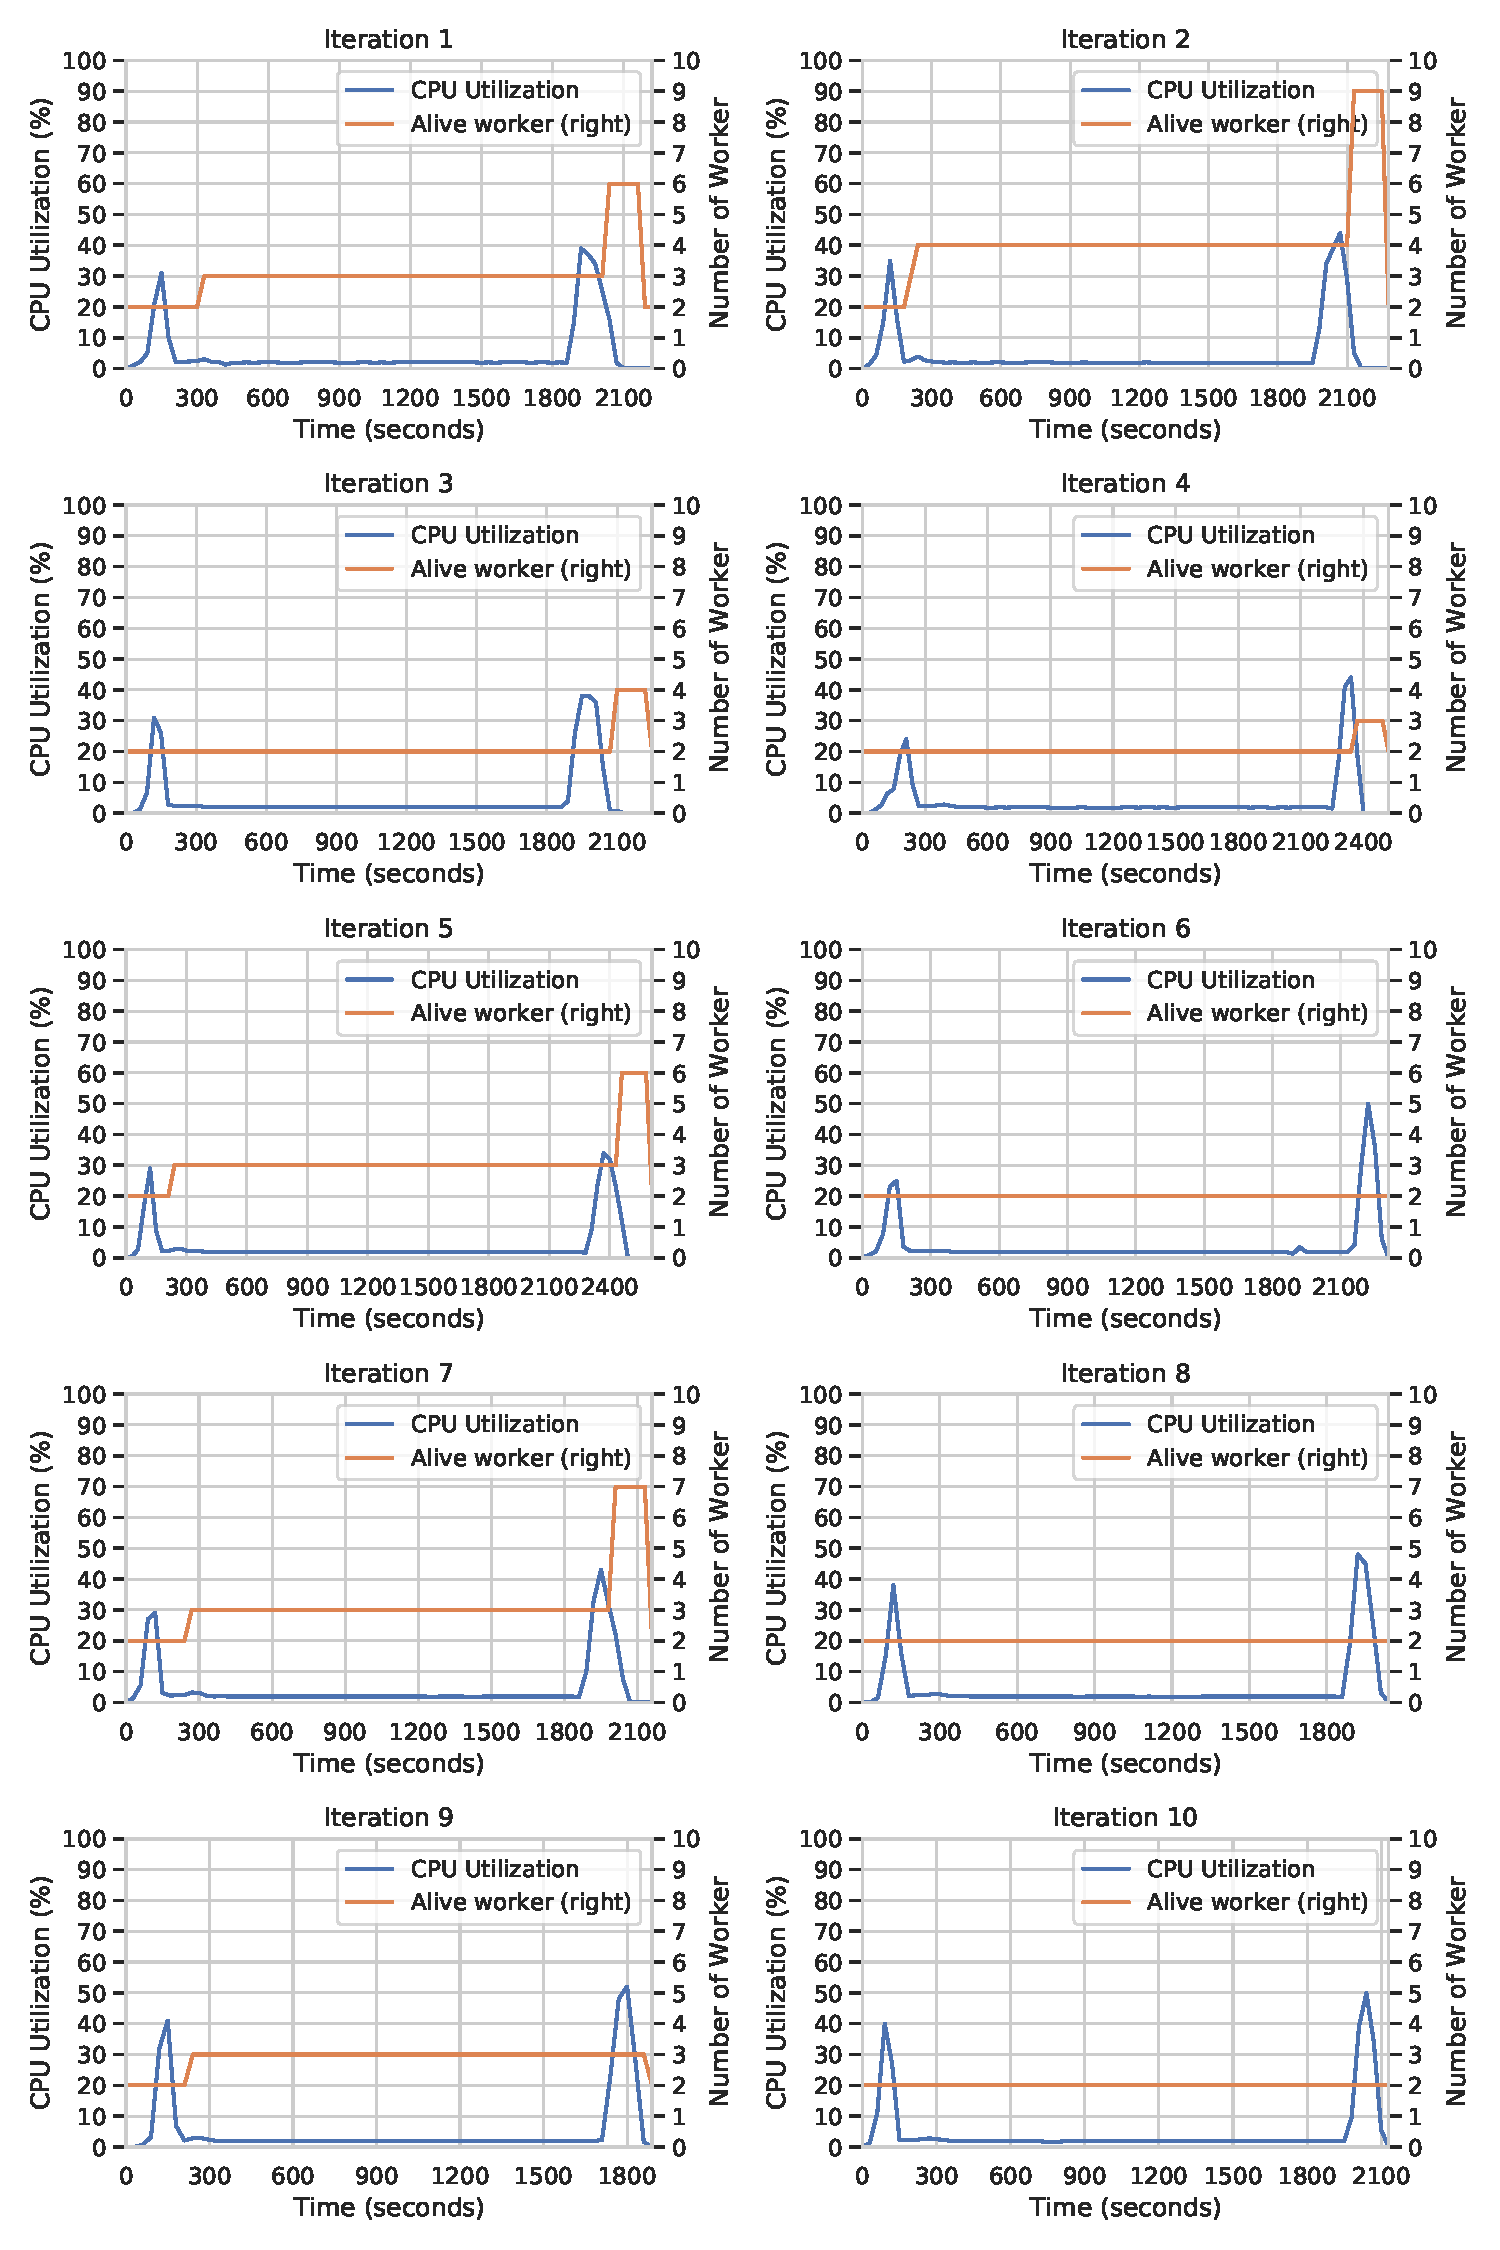
\includegraphics[scale=0.53]{images/07_evaluation/mortgage/mortgage_auto-scaler_performance}
\caption{Basic architecture of a GitLab CI/CD pipeline - Source: Authors own model, based on \cite{Gitlab2020Docs}.}
\label{fig:07_mortgage_static-cpu_results}
\end{figure}
